% Tikz flowchart to show the passage history of 17D and FNV.

%block styles for the chart.
\tikzstyle{parent} = [rectangle, draw, fill=red!20, 
text width=6em, text badly centered, node distance=3cm, inner sep=3pt]
\tikzstyle{intermediate} = [rectangle, draw, fill=orange!20, 
text width=6em, text badly centered, node distance=3cm, inner sep=3pt]
\tikzstyle{derivative} = [rectangle, draw, fill=blue!20, 
text width=6em, text badly centered, node distance=3cm, inner sep=3pt]
\tikzstyle{line} = [draw]
\tikzstyle{arrow} = [thick,->,>=stealth,draw]

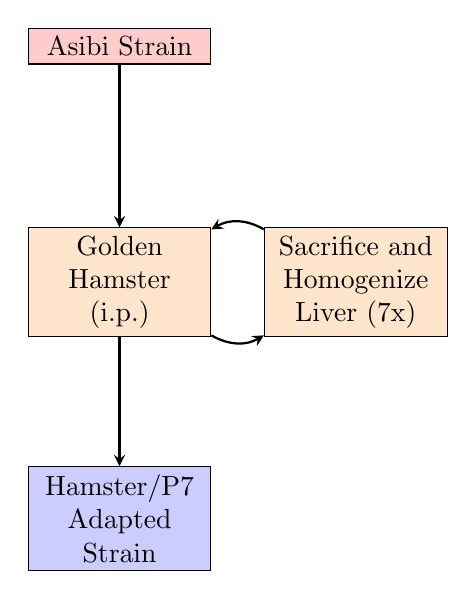
\begin{tikzpicture}[node distance = 4cm]
	%nodes for Asibi
	\node[parent](Asibi){Asibi Strain};
	%nodes for HeLap6
	%\node[intermediate, below left of = Asibi](almostLP){Vero-Purified Asibi};
	%\node[intermediate, below of=almostLP](AsibiLP){Asibi Large Plaque Variant};
	%nodes for Hamp7
	%\node[derivative, below of=AsibiLP](helap6){HeLa p6 Attenuated Strain};
	\node[intermediate, below of=Asibi](hamster){Golden Hamster \\ (i.p.)};
	\node[intermediate, right of=hamster](liver){Sacrifice and \\ Homogenize Liver (7x)};	
	\node[derivative, below of=hamster](hamp7){Hamster/P7 Adapted Strain};

	%edges
	\path[arrow] (Asibi) -- (hamster);
	\path[arrow] (hamster) -- (hamp7);
	\draw[arrow,bend right] (hamster) edge (liver);
	\draw[arrow,bend right] (liver) edge (hamster);
%	\path[arrow] (AsibiLP) -- (helap6)node [midway, left, align=center] (TextNode3) {6x Passage \\ HeLa};
%	\path[arrow] (Asibi) -| (hamp7)node[midway, right, align=center] (TextNode4) {7x Intrahepatic Passage \\ Syrian Golden Hamsters};
	
	
\end{tikzpicture}